% Created 2014-03-06 Thu 22:24
\documentclass[table,smaller]{beamer}
\usepackage[utf8]{inputenc}
\usepackage[T1]{fontenc}
\usepackage{fixltx2e}
\usepackage{graphicx}
\usepackage{longtable}
\usepackage{float}
\usepackage{wrapfig}
\usepackage{rotating}
\usepackage[normalem]{ulem}
\usepackage{amsmath}
\usepackage{textcomp}
\usepackage{marvosym}
\usepackage{wasysym}
\usepackage{amssymb}
\usepackage{hyperref}
\tolerance=1000
\usepackage{tikz}
\usepackage{minted}
\usepackage{fancyvrb}
\usemintedstyle{perldoc}
\definecolor{lightgray}{gray}{0.96}
\setlength{\tabcolsep}{1ex}
\institute{Harvard MIT Data Center}
\usetheme{Warsaw}
\useoutertheme{infolines}
\setbeamercolor{block body}{bg=lightgray}
\titlegraphic{
\includegraphics[width=.75\textwidth]{images/IQSSNewLogo.pdf}}
\setbeamersize{text margin left=2em,text margin right=2em}
\AtBeginSection[]{\begin{frame}<beamer>\frametitle{Topic}\tableofcontents[currentsection]\end{frame}}
\usetheme{default}
\author{}
\date{}
\title{Introduction to SAS}
\hypersetup{
  pdfkeywords={},
  pdfsubject={},
  pdfcreator={Emacs 24.3.1 (Org mode 8.2.5h)}}
\begin{document}

\maketitle
\begin{frame}{Outline}
\tableofcontents
\end{frame}



\section{Introduction}
\label{sec-1}

\begin{frame}[label=sec-1-1]{Documents for Today}
\begin{itemize}
\item Log in
\begin{itemize}
\item USERNAME: dataclass
\item PASSWORD: dataclass
\end{itemize}
\item Find class materials at \url{http://j.mp/sas-intro}
\item Includes data, presentation slides, exercises
\item Extract (right-click ==> WinZipCopy ==> Extract here) and move materials to your desktop!
\end{itemize}
\end{frame}
\begin{frame}[label=sec-1-2]{Workshop Description}
\begin{itemize}
\item This is an INTRODUCTION to SAS -- assumes no knowledge of SAS!
\item Not appropriate for people already well familiar with SAS
\item Learning Objectives:
\begin{itemize}
\item Import and export data in a varity of formats
\item Create and use variable and value labels
\item Perform basic data manipulation
\item Compoute descriptive statistics
\item Wrap-up
\end{itemize}
\end{itemize}
\end{frame}
\begin{frame}[label=sec-1-3]{Why SAS?}
\begin{itemize}
\item If you know SAS, it is likely you will not need any other software packages
\item Among the most powerful statistical software packages available
\item Great user community: macros, websites, etc.
\item Free online documentation:
\item \url{http://support.sas.com/documentation/93/index.html}
\end{itemize}
\end{frame}
\begin{frame}[label=sec-1-4]{SAS history}
SAS was first developed in the 1970's. The world was a lot different then!
(Image source: \url{http://en.wikipedia.org/wiki/Moore's_law})
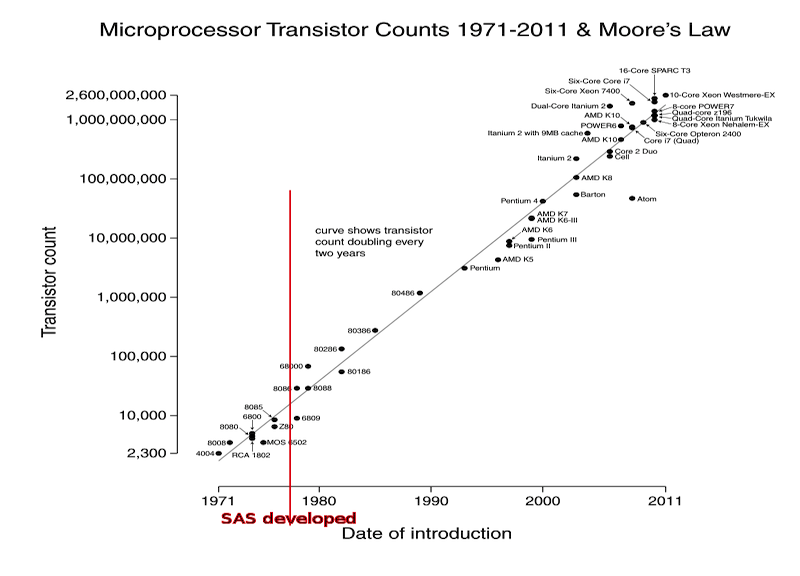
\includegraphics[width=.9\linewidth]{./images/SASinContext.png}
\end{frame}
\begin{frame}[label=sec-1-5]{The SAS Environment}
\begin{itemize}
\item Five basic SAS windows:
\begin{itemize}
\item Results
\item Explorer
\item Editor
\item Log
\item Output
\end{itemize}
\item Set up your SAS window so it fits your own preferences
\item Viewing options (Windows only):
\begin{itemize}
\item Window > Tile Vertically
\end{itemize}
\end{itemize}
\end{frame}
\begin{frame}[fragile,label=sec-1-6]{SAS Basics}
 \begin{itemize}
\item SAS has point-and-click interfaces, but most users write command-driven SAS programs
\item Command syntax is not case sensitive, but file names may be
\item Commands can run on multiple lines (but you can't split words across lines)
\item Follow every command with RUN ;
\item Comments can be written as:
\begin{itemize}
\item \verb~/* comment comment comment */~ OR
\item \verb~* comment comment comment;~
\end{itemize}
\end{itemize}
\end{frame}

\section{Data Import and Export}
\label{sec-2}

\begin{frame}[label=sec-2-1]{Working With SAS Data}
\begin{itemize}
\item SAS data sets are stored in files on your hard drive, usually with the extension ".sas7bdat"
\item Under Unix/Linux SAS data file names must be all lowercase--best to observe this restriction on Windows as well
\item In SAS there is no concept of "opening" a data set--Instead we use \emph{libraries} to point to directories on the hard drive that contain SAS data sets
\item Unless you specify otherwise, SAS copies your data temporarily in a library called "work"
\item The work library is temporary, so
\begin{itemize}
\item use the work library for temporary data sets
\item create and use your own library for any data you wish to save
\end{itemize}
\end{itemize}
\end{frame}
\begin{frame}[fragile,label=sec-2-2]{Libraries and Datasets}
 Tell SAS where our data is on our hard drive by creating a library -- I'm going to name my library \emph{introSAS} and point SAS to the \emph{dataSets} folder

\vspace{-.75em} \begin{columns} \column{.90\linewidth} \begin{block}{}
\begin{minted}[fontsize=\footnotesize]{c}
/* initialize a SAS library in the dataSets folder */
LIBNAME introSAS "C:/Users/dataclass/Desktop/SASintro/dataSets";
RUN;
/* list sas datasets in the introSAS library / dataSets folder */
PROC DATASETS library=introSAS;
RUN;
/* initialize a SAS library in the SASintroLib folder */
LIBNAME mylib "C:/Users/dataclass/Desktop/SASintro/SASintroLib";
RUN;
/* copy pubschool to the "work" library */
DATA pubschool;
     SET "C:/Users/dataclass/Desktop/SASintro/dataSets/pubschool";
RUN;
\end{minted}
\end{block} \end{columns} \vspace{.25em}

\begin{itemize}
\item The DATA command is actually saving our dataset as a new  file called "pubschool" in the "work" library
\item The SET command is just telling SAS what dataset to save
\end{itemize}
\end{frame}
\begin{frame}[fragile,label=sec-2-3]{What if my file is not a SAS file?}
 In SAS "import" means "convert to SAS format, copy to library/folder"

\begin{itemize}
\item Import Stata files with \emph{dbms=dta}
\end{itemize}
\vspace{-.75em} \begin{columns} \column{.90\linewidth} \begin{block}{}
\begin{minted}[fontsize=\footnotesize]{c}
/* import from stata format */
PROC IMPORT out = pubschool
    DATAFILE = "C:/Users/dataclass/Desktop/SASintro/dataSets/pubschool.dta"
    DBMS = dta replace;
RUN;
\end{minted}
\end{block} \end{columns} \vspace{.25em}

\begin{itemize}
\item Importing ASCII files with (e.g.) \emph{dbms=csv}
\end{itemize}
\vspace{-.75em} \begin{columns} \column{.90\linewidth} \begin{block}{}
\begin{minted}[fontsize=\footnotesize]{c}
/* import csv file */
PROC IMPORT out = pubschool
     DATAFILE = "C:/Users/dataclass/Desktop/SASintro/dataSets/pubschool.csv"
     DBMS = csv   replace;
     GETNAMES = yes;
     DATAROW = 2;
RUN;
\end{minted}
\end{block} \end{columns} \vspace{.25em}
\end{frame}
\begin{frame}[fragile,label=sec-2-4]{Where is my data?}
 You can "view" you data in a couple of ways:
\begin{itemize}
\item Proc contents
\end{itemize}
\vspace{-.75em} \begin{columns} \column{.90\linewidth} \begin{block}{}
\begin{minted}[fontsize=\footnotesize]{c}
/* list contents of pubschool data */
PROC CONTENTS data = pubschool;
     TITLE "Public school contents";
RUN;
\end{minted}
\end{block} \end{columns} \vspace{.25em}

\begin{itemize}
\item Data viewer
\begin{enumerate}
\item Go to explorer
\item Select your "work" library
\item Click on your dataset (opens in SAS Universal Viewer)
\end{enumerate}
\item Your dataset is named in the library as "pubschool" because that's what you named it when you originally opened the dataset
\end{itemize}
\end{frame}
\begin{frame}[fragile,label=sec-2-5]{How do I get my data out of SAS?}
 In SAS "export" means "convert to a non-SAS format"

\begin{itemize}
\item Exporting CSV files:
\end{itemize}
\vspace{-.75em} \begin{columns} \column{.90\linewidth} \begin{block}{}
\begin{minted}[fontsize=\footnotesize]{c}
/* export to .csv */
PROC EXPORT data = introSAS.ntcs
     OUTFILE = "C:/Users/dataclass/Desktop/SASintro/SASintroLib/NeighCrime_NEW_EXPORT.csv"
     DBMS = csv;
RUN;
\end{minted}
\end{block} \end{columns} \vspace{.25em}

\begin{itemize}
\item Exporting tab delimited files:
\end{itemize}
\vspace{-.75em} \begin{columns} \column{.90\linewidth} \begin{block}{}
\begin{minted}[fontsize=\footnotesize]{c}
/* export to tab delimited */
PROC EXPORT data = introSAS.ntcs
     OUTFILE = "C:/Users/dataclass/Desktop/SASintro/SASintroLib/NeighCrime_NEW_EXPORT.txt"
     DBMS = tab;
RUN;
\end{minted}
\end{block} \end{columns} \vspace{.25em}
\end{frame}

\begin{frame}[label=sec-2-6]{Exercise 1: Importing Data}
\begin{enumerate}
\item Create a library named "mylib" in the SASintroLib folder if it doesn't already exist
\item Import the Stata file, "ntcs.dta" to the mylib library
\item Import the ASCII file, "ntcs.csv" to the mylib library
\item Use "proc datasets" to list the datasets in the mylib libary
\item Use "proc contents" to review the data you imported in step 2
\end{enumerate}
\end{frame}
\section{Descriptive Statistics}
\label{sec-3}

\begin{frame}[fragile,label=sec-3-1]{Means, standard deviations, etc.}
 Compute averages for q1 and q2 using proc means
\vspace{-.75em} \begin{columns} \column{.90\linewidth} \begin{block}{}

\begin{minted}[fontsize=\footnotesize]{c}
/* means of vars q1 and q2 */
PROC MEANS data = pubschool;
     VAR q1 q2;
     TITLE "Public school means";
RUN;
\end{minted}

\end{block} \end{columns} \vspace{.25em}

Compute averages for q1 separately by timezone
\vspace{-.75em} \begin{columns} \column{.90\linewidth} \begin{block}{}

\begin{minted}[fontsize=\footnotesize]{c}
/* means separatly by timezone */
/* need to sort first */
PROC SORT data = pubschool;
    by timezone;
RUN;

PROC MEANS data = pubschool;
    by timezone;
    VAR q1;
    TITLE "Public school means by timezone";
RUN;
\end{minted}

\end{block} \end{columns} \vspace{.25em}
\end{frame}
\begin{frame}[fragile,label=sec-3-2]{Frequency Tables}
 Frequency tables for q1 and q2 using proc freq
\vspace{-.75em} \begin{columns} \column{.90\linewidth} \begin{block}{}
\begin{minted}[fontsize=\footnotesize]{c}
/* counts of responses to q3, q4, and q5 */
PROC FREQ data = pubschool;
     TABLE q3 q4 q5;
     TITLE "Public school frequencies";
RUN;
\end{minted}
\end{block} \end{columns} \vspace{.25em}

Frequency tables for q1 by timezone
\vspace{-.75em} \begin{columns} \column{.90\linewidth} \begin{block}{}
\begin{minted}[fontsize=\footnotesize]{c}
/* counts by timezone */
PROC FREQ data = pubschool;
     TABLE q3*timezone;
     TITLE "Public school frequencies";
RUN;
\end{minted}
\end{block} \end{columns} \vspace{.25em}
\end{frame}

\begin{frame}[fragile,label=sec-3-3]{Correlation and Regression}
 We're interested in looking at the relationship between City Crime Rate (C\_CRIMRT) and Percent of High School Grads in the City (C\_HSGRAD)

\vspace{-.75em} \begin{columns} \column{.90\linewidth} \begin{block}{}
\begin{minted}[fontsize=\footnotesize]{c}
/* Scatterplot of relationship between high school
   graduation rate and crime rate */
PROC GPLOT data = introSAS.ntcs;
     PLOT    C_HSGRAD * C_CRIMRT;
     TITLE "Percent of High School Graduates and Crime Rates";
RUN;
/* correlation between graduation and crime rates */
PROC CORR data = introSAS.ntcs;
   VAR     C_HSGRAD C_CRIMRT;
      TITLE "Percent of High School Graduates and Crime Rates";
RUN;
 /* Regression predicting crime rate */
PROC REG data = introSAS.ntcs;
     MODEL C_CRIMRT = C_HSGRAD C_PERCAP C_POVRTY;
     TITLE "Percent of High School Graduates and Crime Rates";
RUN;
\end{minted}
\end{block} \end{columns} \vspace{.25em}
\end{frame}

\begin{frame}[label=sec-3-4]{Exercise 2: Correlation and regression}
Use the ntcs data set

\begin{enumerate}
\item Take a look around the ntcs dataset and identify an outcome you'd like to predict and few variables (4-6) that you believe would serve as relevant predictor variables
\item Run relevant descriptive statistics on your variables and look at histograms and scatterplots
\item Test correlations leading up to ultimately testing a regression
\item Run and interpret a regression using your selected variables
\end{enumerate}
\end{frame}
\section{Variable and Value Labels}
\label{sec-4}

\begin{frame}[label=sec-4-1]{Variable and Value Labels}
\begin{itemize}
\item Variable labels refer to the titles associated with each variable
\item Value labels refer to the titles you assign to the different levels (i.e., values) of each variable
\item EXAMPLE:
\begin{itemize}
\item Variable name: Marital
\item Variable label: Marital status of participant
\item Value labels: 1 = Married, 2 = Separated, 3= Divorced, 4 = Single, etc.
\end{itemize}
\end{itemize}
\end{frame}
\begin{frame}[fragile,label=sec-4-2]{Variable Labels}
 Adding variable labels is a \emph{data step} command:

\vspace{-.75em} \begin{columns} \column{.90\linewidth} \begin{block}{}
\begin{minted}[fontsize=\footnotesize]{c}
/* copy pubschool to pubschool2 and label resp and status */
DATA pubschool2;
  SET pubschool;
  LABEL
     resp = "Participant Identifier"
     status = "Did participant complete survey?"
RUN;
/* Check output */
PROC CONTENTS data = pubschool2;
   TITLE "pubschool2 contents";
RUN;
\end{minted}
\end{block} \end{columns} \vspace{.25em}
\end{frame}
\begin{frame}[fragile,label=sec-4-3]{Creating Value Labels}
 Creating value labels is a \emph{proc} command
\begin{itemize}
\item Start by creating the label format
\end{itemize}
\vspace{-.75em} \begin{columns} \column{.90\linewidth} \begin{block}{}
\begin{minted}[fontsize=\footnotesize]{c}
/* create value label named q1label */
PROC FORMAT;
 VALUE q1label
       1 = "best"
       2 = "top 5"
       3 = "top 10"
       4 = "top 20"
       5 = "Bottom 80"
       9 = "Don't know";
RUN;
\end{minted}
\end{block} \end{columns} \vspace{.25em}
\end{frame}
\begin{frame}[fragile,label=sec-4-4]{Using Value labels}
 Now we can use this value scheme creating tables,output, etc.

\vspace{-.75em} \begin{columns} \column{.90\linewidth} \begin{block}{}
\begin{minted}[fontsize=\footnotesize]{c}
/* display fequencies, using value labels */
PROC FREQ data = pubschool;
      TABLES q1;
      FORMAT q1 q1label.;
RUN;
/* NOTE: There is a "." after q1label. This alerts SAS
 that you're referring to a value scheme Saving Value
 Labels in your Dataset */
\end{minted}
\end{block} \end{columns} \vspace{.25em}

We can also save a value label in a data set,
\vspace{-.75em} \begin{columns} \column{.90\linewidth} \begin{block}{}
\begin{minted}[fontsize=\footnotesize]{c}
/* add value label to SAS data set */
PROC DATASETS library = work;
     MODIFY pubschool2;
format     q1 q1label.;
RUN;
/* confirm that our formats were correctly applied: */
PROC FREQ data = pubschool2;
TABLES    q1 q3;
RUN;
\end{minted}
\end{block} \end{columns} \vspace{.25em}
\end{frame}
\begin{frame}[fragile,label=sec-4-5]{Dropping and Renaming Variables}
 Keeping a subset  of variables is simple--use the "drop" or "keep" command:

\vspace{-.75em} \begin{columns} \column{.90\linewidth} \begin{block}{}
\begin{minted}[fontsize=\footnotesize]{c}
/* create new dataset "pubschoolKeep" with only q1-q5 */
DATA   pubschoolKeep (keep = q1 q2 q3 q4 q5);
     SET pubschool;
RUN;
/* create new dataset pubschoolDrop, excluding q1-q5 */
DATA   pubschoolDrop       (drop = q1 q2 q3 q4 q5);
     SET pubschool;
RUN;
\end{minted}
\end{block} \end{columns} \vspace{.25em}


Renameing variables is done in a data step: just put the rename syntax right after your data command

\vspace{-.75em} \begin{columns} \column{.90\linewidth} \begin{block}{}
\begin{minted}[fontsize=\footnotesize]{c}
/* change the name of q2 to q2newName */
DATA pubschool2 (rename = (q2 = q2newName));
     SET pubschool2;
RUN;
/* View the dataset: */
PROC CONTENTS data = pubschool2;
RUN;
\end{minted}
\end{block} \end{columns} \vspace{.25em}
\end{frame}
\begin{frame}[fragile,label=sec-4-6]{SAS variable names}
 \begin{itemize}
\item Must be \verb~<=~ 32 characters in length
\item Must start with a letter or underscore
\item Can contain only numbers, letters or underscores
\begin{itemize}
\item No special characters: \verb~@#$%^&*~
\end{itemize}
\item Can contain upper and lowercase letters
\end{itemize}
\end{frame}
\section{Data Manipulation}
\label{sec-5}

\begin{frame}[fragile,label=sec-5-1]{Logic Statements Useful For Data Manipulation}
 \begin{description}
\item[{\verb~=~ (EQ)}] equal to
\item[{\verb~^=~ (NE)}] not equal to
\item[{\verb~>~ (GT)}] greater than
\item[{\verb~<~ (LT)}] less than
\item[{\verb~>=~ (GE)}] greater than or equal to
\item[{\verb~<=~ (LE)}] less than or equal to
\item[{\verb~&~ (AND)}] and
\item[{\verb~|~ (OR)}] or
\end{description}
\end{frame}

\begin{frame}[fragile,label=sec-5-2]{Generate New Variables}
 A data command - simply put new variable name followed by variable condition.
\vspace{-.75em} \begin{columns} \column{.90\linewidth} \begin{block}{}
\begin{minted}[fontsize=\footnotesize]{c}
DATA pubschool2;
    SET pubschool;
    /* create variable "myvar" equal to q1 */
    myvar = q1;
    /* create variable newvar2 equal to 1 */
    newvar2 = 1;
RUN;
\end{minted}
\end{block} \end{columns} \vspace{.25em}

Create new variable based on values of existing variable

\vspace{-.75em} \begin{columns} \column{.90\linewidth} \begin{block}{}
\begin{minted}[fontsize=\footnotesize]{c}
/* generate newvar4 based on q1 */
DATA pubschool2;
    SET pubschool;
    if q1=1 then newvar3=1;
    else if q1=2 then newvar3=2;
    else if q1=3 then newvar3=3;
    else if q1=4 then newvar3=4;
    else newvar3=.;
RUN;
\end{minted}
\end{block} \end{columns} \vspace{.25em}
\end{frame}

\begin{frame}[fragile,label=sec-5-3]{Saving Subsets of Data}
 Subsets are created with in a \emph{data step}

\begin{itemize}
\item Create a subset of data including only participants who had a child attending a public school
\end{itemize}

\vspace{-.75em} \begin{columns} \column{.90\linewidth} \begin{block}{}
\begin{minted}[fontsize=\footnotesize]{c}
/* keep only rows where q10 is 1 */
DATA CurrentPublic;
     SET pubschool;
     if q10=1;
RUN;
\end{minted}
\end{block} \end{columns} \vspace{.25em}

\begin{itemize}
\item Create a subset of data including participants in timezone 1 or 2
\end{itemize}
\vspace{-.75em} \begin{columns} \column{.90\linewidth} \begin{block}{}
\begin{minted}[fontsize=\footnotesize]{c}
/* keep only rows where timezone is 1 or 2 */
DATA CurrentPublic;
     SET pubschool;
     if timezone=1 | timezone=2;
RUN;
\end{minted}
\end{block} \end{columns} \vspace{.25em}
\end{frame}

\begin{frame}[label=sec-5-4]{Missing Values}
\begin{itemize}
\item SAS's symbol for a missing value is "."
\item SAS interprets "." as a small value
\item Need to be aware of this when you are manipulating data!
\begin{itemize}
\item What will happen when you use the < or <= commands?
\end{itemize}
\end{itemize}
\end{frame}
\begin{frame}[label=sec-5-5]{Exercise 3: Data Manipulation}
Use the ntcs.sas7bdat

\begin{enumerate}
\item Attach variable labels using the following codebook:
\begin{itemize}
\item REGION =  "Region in United States"
\item CITY = "Name of City and State"
\end{itemize}
\item Create formats in SAS using the codebook below:
\begin{itemize}
\item C\_SOUTH: 1 = Southern City, 0=Non-Southern City
\item C\_WEST: 1=Western City 0=Non-Western City
\end{itemize}
\item Run "proc freq" on C\_SOUTH and C\_WEST and use formats from step 2
\item Assign the formats for C\_SOUTH and C\_WEST permanently in your ntcs dataset
\item Confirm with "proc freq" that your labels were correctly assigned
\item Generate new variables based on the city-level crime variables "C\_MURDRT" and "C\_ROBBRT". Choose values on which to dichotomize each variable and create new variables that have a score of "1" if the original variable is above that value, and a score of "0" otherwise.
\item Confirm that your new variables were properly created using "proc freq"
\end{enumerate}
\end{frame}
\section{Wrap-up}
\label{sec-6}


\begin{frame}[label=sec-6-1]{Help us make this workshop better!}
\begin{itemize}
\item Please take a moment to fill out a very short feedback form

\item These workshops exist for you – tell us what you need!

\item \url{http://tinyurl.com/akyvzle}
\end{itemize}
\end{frame}
\begin{frame}[label=sec-6-2]{Other Services Available}
Institute for Quantitative Social Science
\begin{itemize}
\item www.iq.harvard.edu
\end{itemize}
Computer labs
\begin{itemize}
\item www.iq.harvard.edu/facilities
\end{itemize}
Research Technology Consulting
\begin{itemize}
\item www.iq.harvard.edu/researchconsulting
\end{itemize}
Training
\begin{itemize}
\item \url{http://projects.iq.harvard.edu/rtc/filter_by/workshops}
\end{itemize}
\end{frame}
\begin{frame}[label=sec-6-3]{Additional Resources}
How do I get SAS?
\begin{itemize}
\item Your Department IT
\item HMDC labs
\item RCE (Research Computing Environment)
\item Buy it: educational or grad plan
\end{itemize}

The RCE
\begin{itemize}
\item Research Computing Enviroment (RCE) service available to
Harvard \& MIT users
\item www.iq.harvard.edu/research\_computing
\item Supplies persistent desktop environment accessible from
any computer with an internet connection
\item Includes SAS, Stata, R etc.
\end{itemize}
\end{frame}
% Emacs 24.3.1 (Org mode 8.2.5h)
\end{document}